\chapter{Results}

In this project, we have total of seven metrics that we wanted to classify using machine learning model. The seven metrics are

\begin{enumerate}
    \item ALUTs
    \item DSP Blocks
    \item Logic Utilization
    \item Memory Bits
    \item Registers
    \item Kernel Fmax
    \item RAM Blocks
\end{enumerate}

The following three figures, Figure \ref{figure:dfsin_roc_curve}, \ref{figure:dfmul_roc_curve} and \ref{figure:dfadd_roc_curve}, showed the ROC curve of all algorithms on how they performed for the metric classifications in each benchmark.

\begin{figure}[H]
\centering
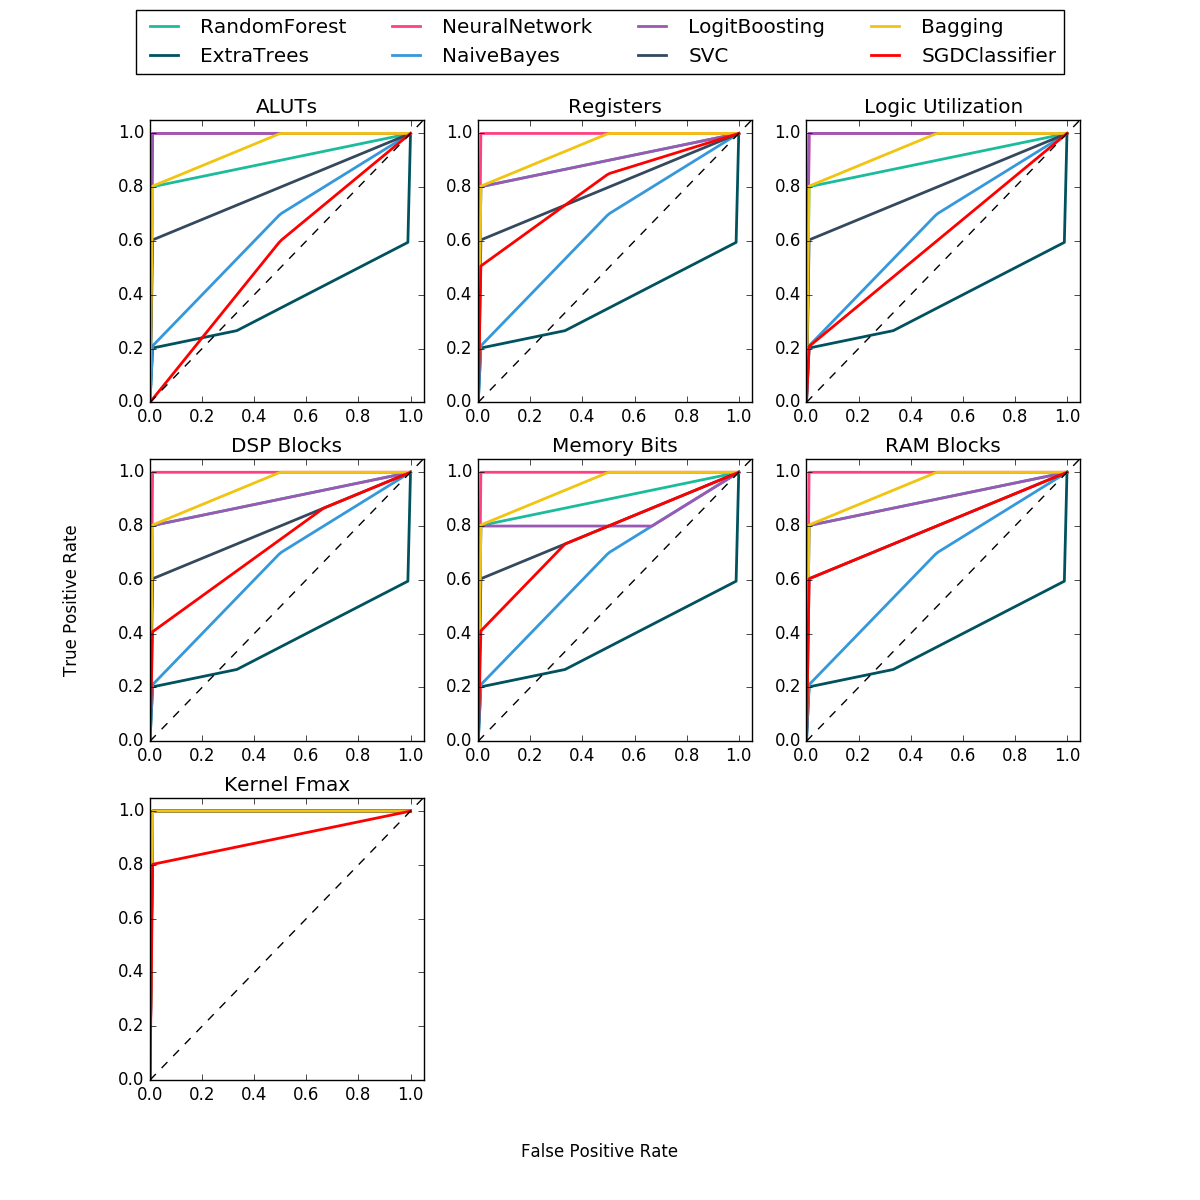
\includegraphics[scale=0.4]{dfsin_roc_curve.png}
\caption{ROC curve for dfsin benchmarks}
\label{figure:dfsin_roc_curve}
\end{figure}

\begin{figure}[H]
\centering
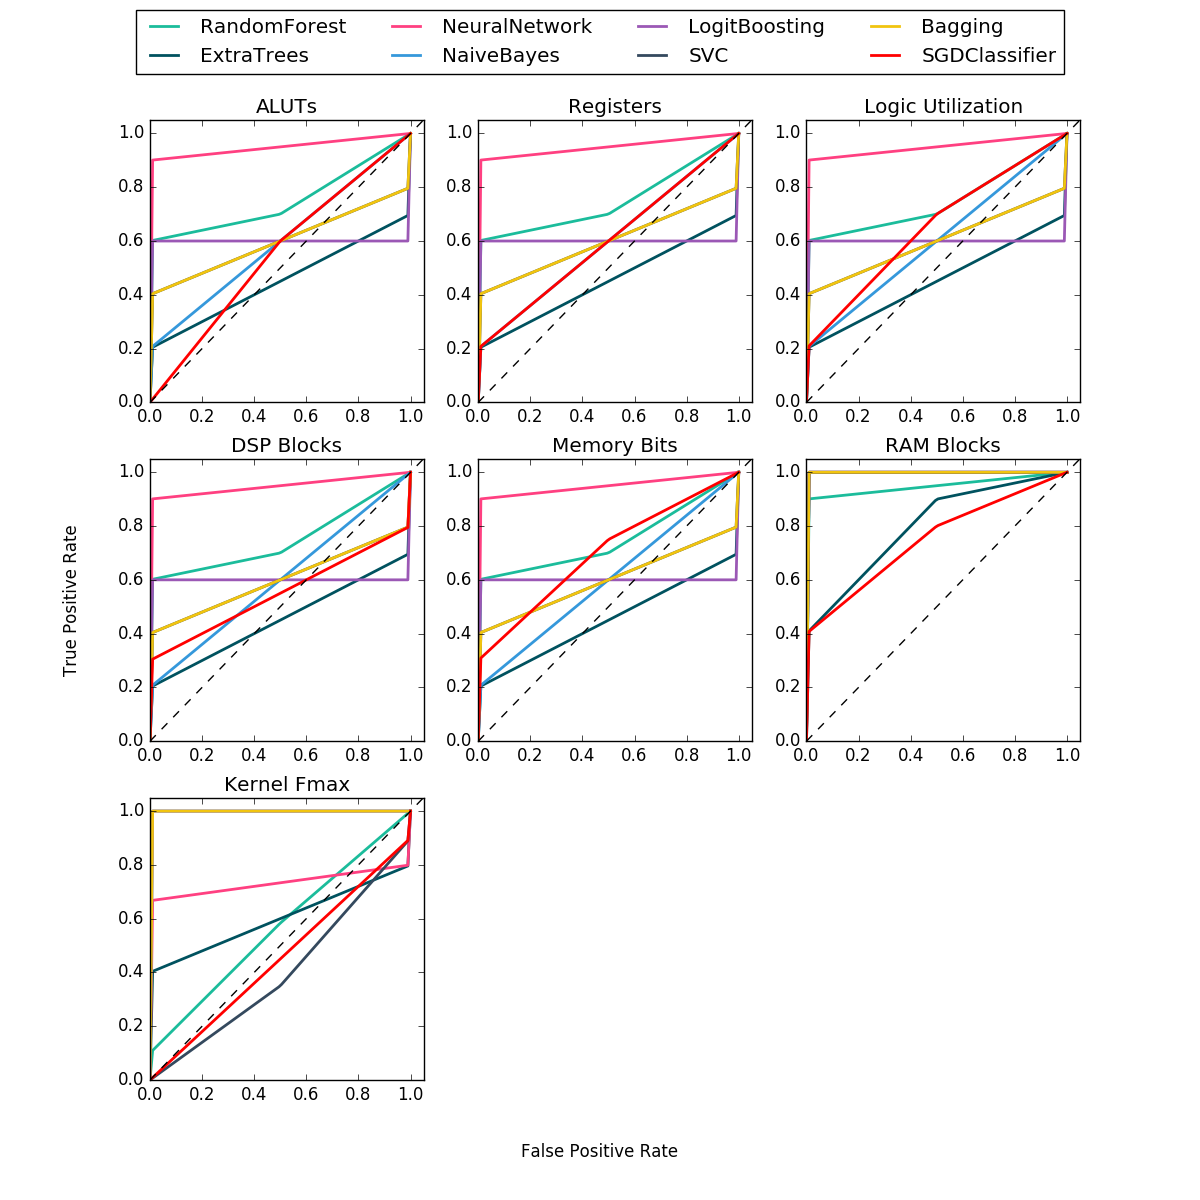
\includegraphics[scale=0.4]{dfmul_roc_curve.png}
\caption{ROC curve for dfmul benchmarks}
\label{figure:dfmul_roc_curve}
\end{figure}

\begin{figure}[H]
\centering
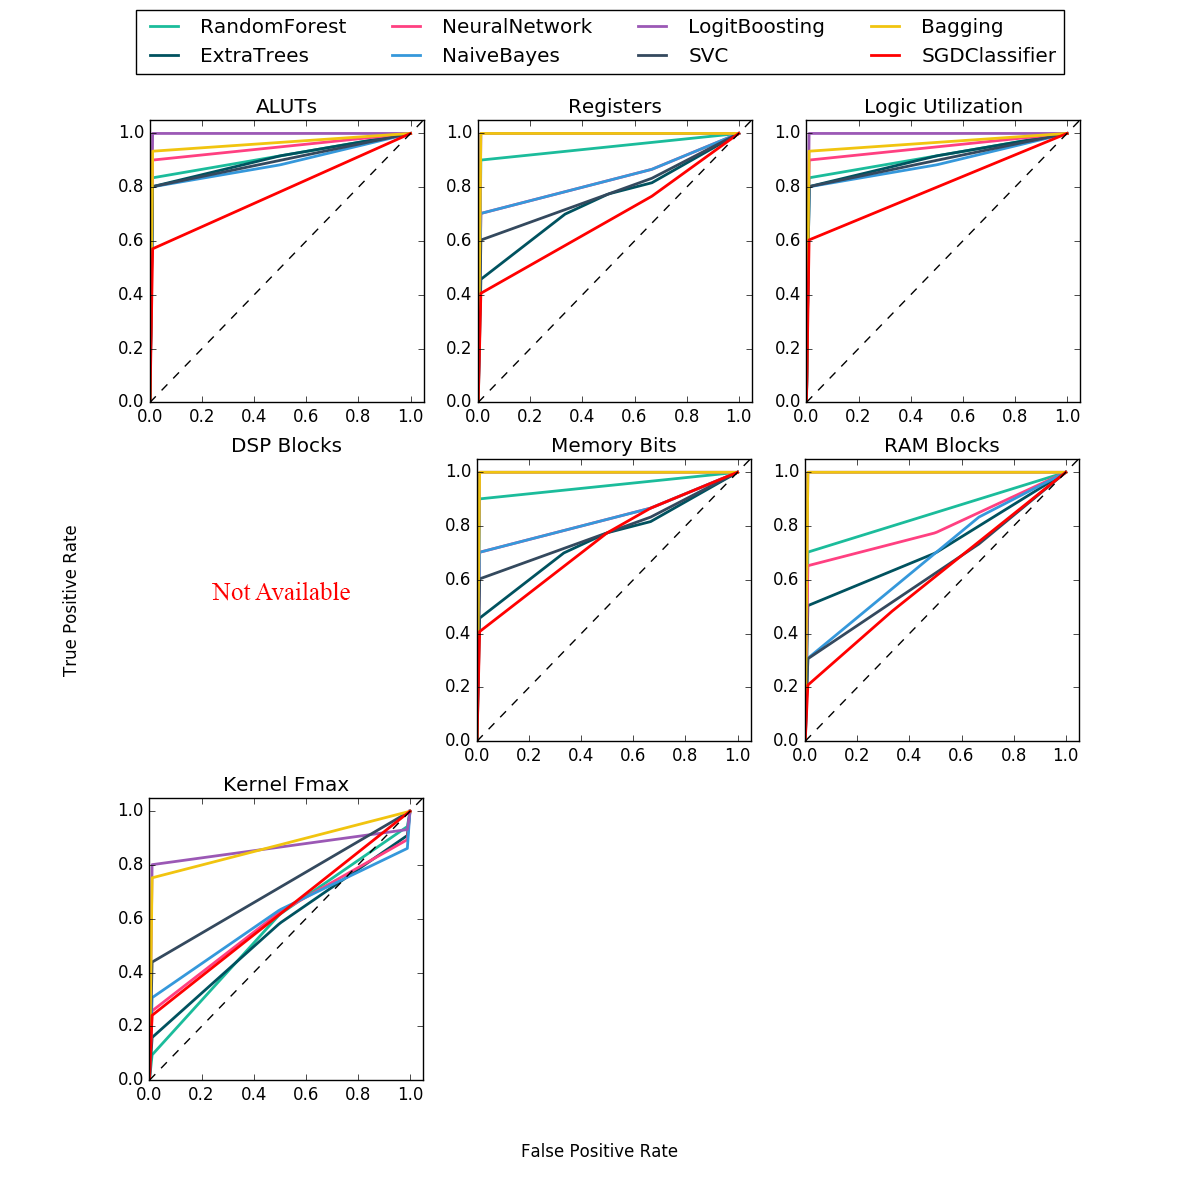
\includegraphics[scale=0.4]{dfadd_roc_curve.png}
\caption{ROC curve for dfadd benchmarks}
\label{figure:dfadd_roc_curve}
\end{figure}

The results are analysed for individual metrics. To get clearer analysis, AUC score will be used to compare the performance of the classifiers in each classification.

\section{Classification of ALUTS}
\begin{figure}[h!]
\centering
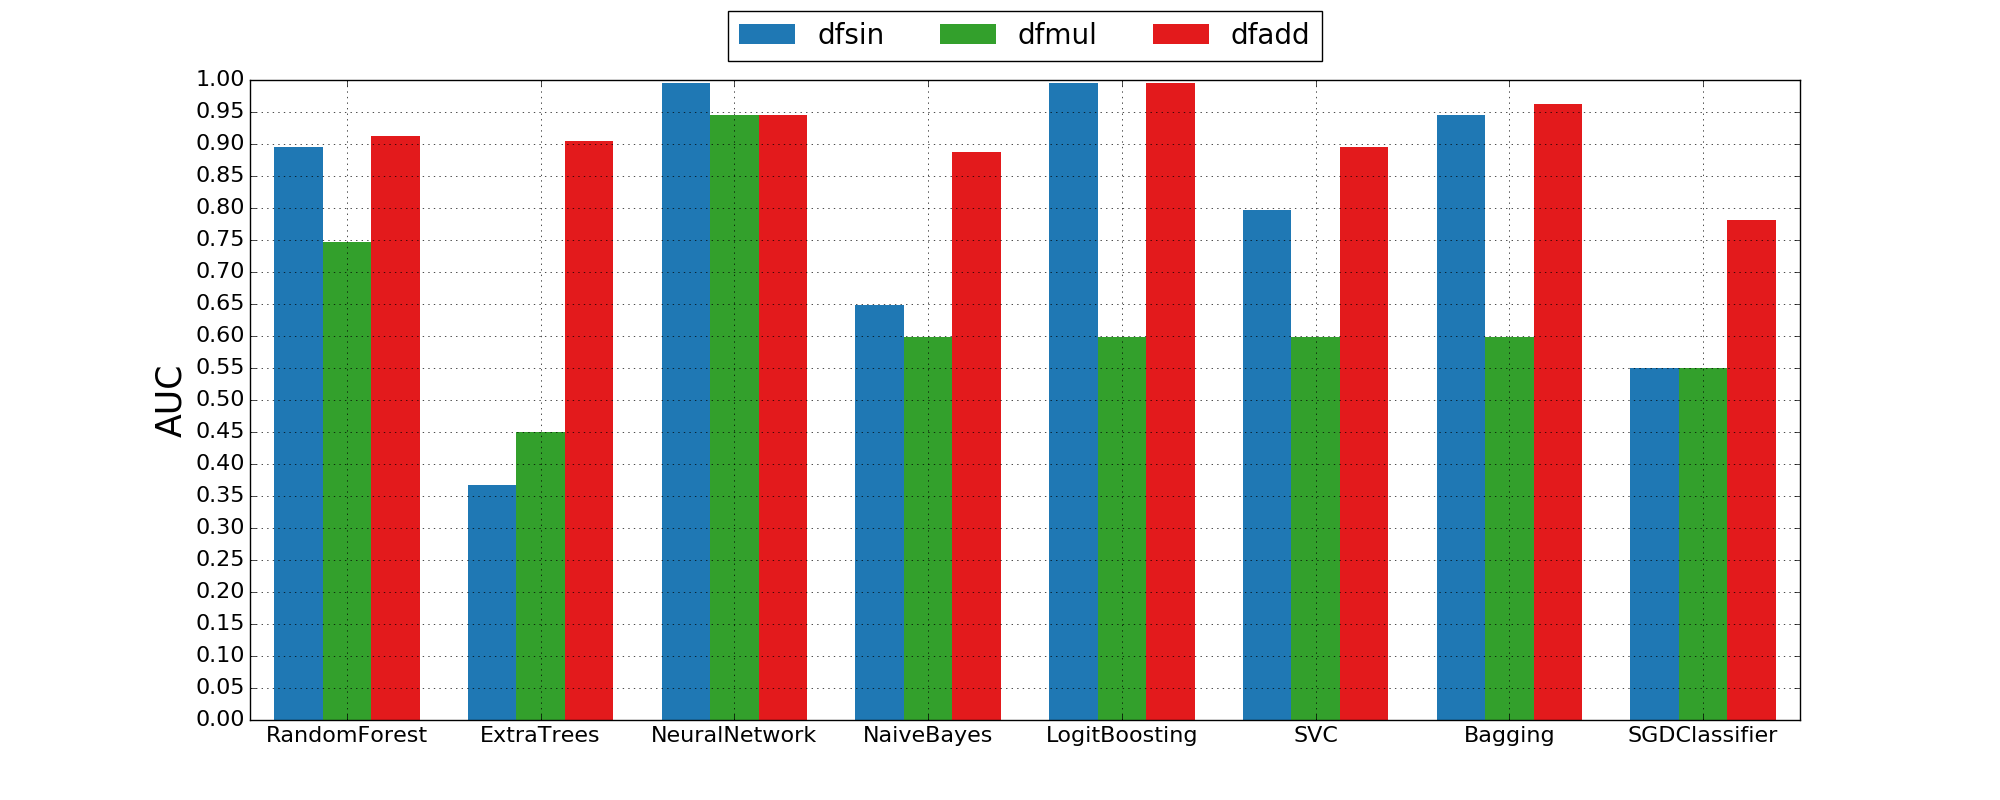
\includegraphics[scale=0.3]{ALUTs_auc_plot.png}
\caption{AUC bar chart for ALUTs}
\label{figure:ALUTs_auc_plot}
\end{figure}

Figure \ref{figure:ALUTs_auc_plot} showed the AUC score for all algorithms that are used to classify ALUTs. Performance variations can be seen clearly. NeuralNetwork classifier has the highest average AUC score of 0.963. ExtraTrees achieved the average AUC score of 0.57 which is the lowest among the eight classifiers and it is followed by SGDClassifier. The reason why SGDClassifier performed poorly is because the data are not linearly separable. Most impressive fact is that RandomForest performed better than ExtraTrees even though ExtraTrees is expected to perform better due to its true more randomness. This happened due to the fact that the data sets and the number of features are relatively small. With the increase of data sets, ExtraTrees should perform better than RandomForest.

\section{Classification of Logic Utilization}

\begin{figure}[h!]
\centering
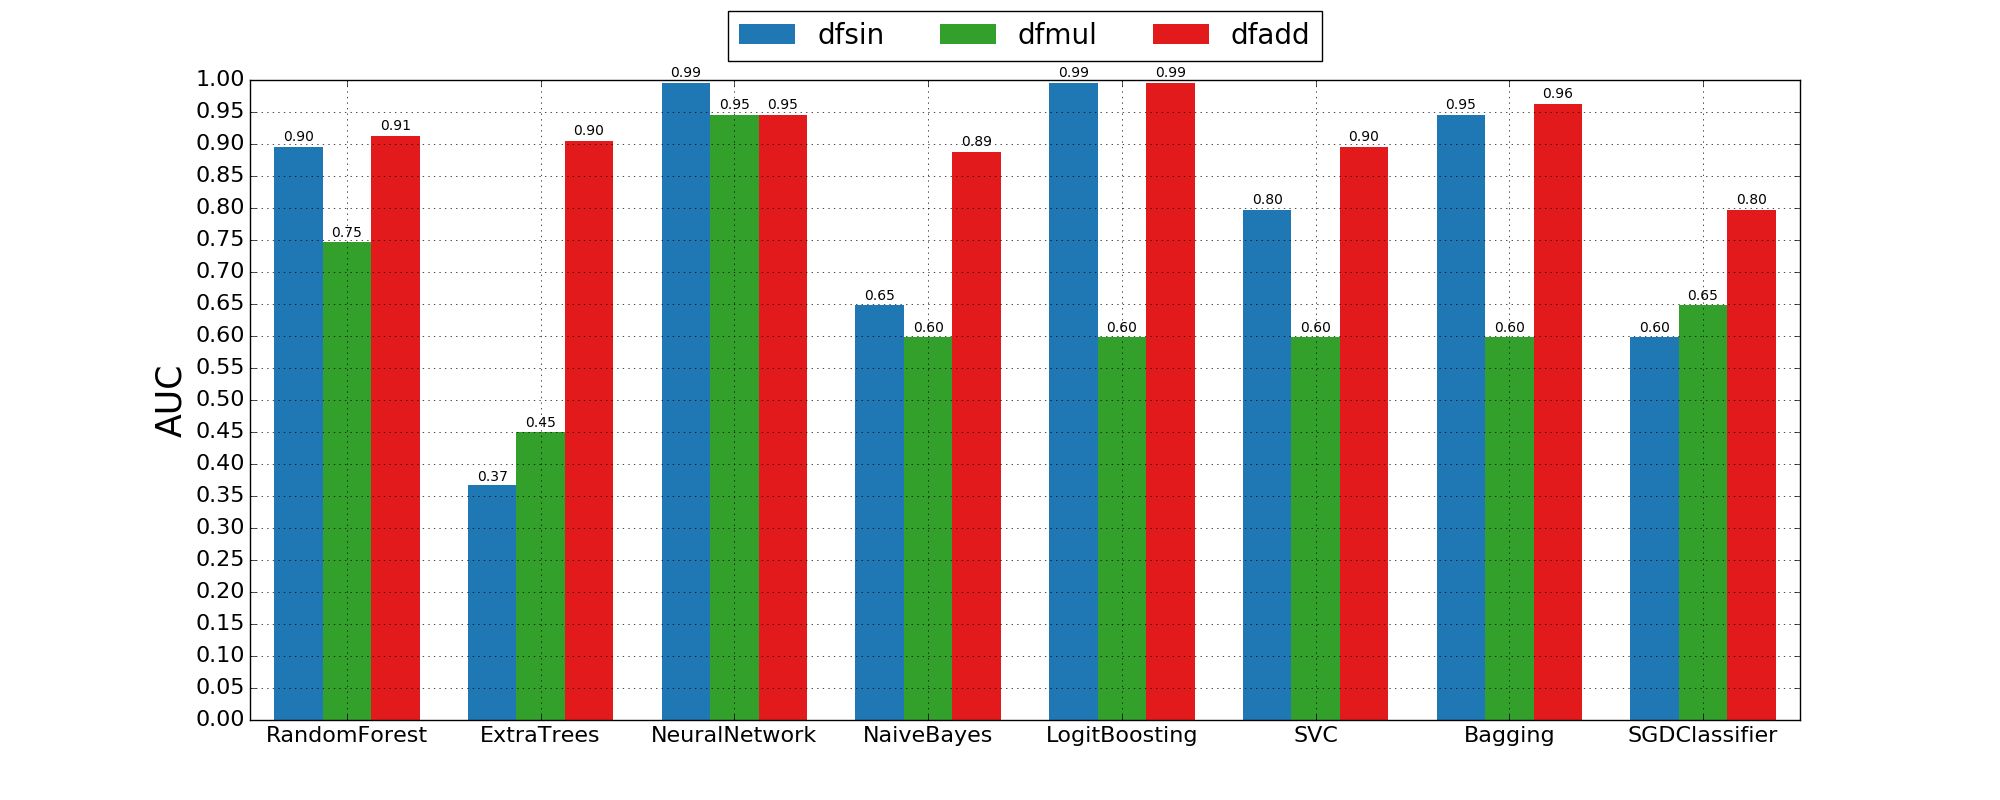
\includegraphics[scale=0.3]{LogicUtilization_auc_plot.png}
\caption{AUC bar chart for Logic Utilization}
\label{figure:LogicUtilization_auc_plot}
\end{figure}

Figure \ref{figure:LogicUtilization_auc_plot} showed the AUC score for all algorithms that are used to classify Logic Utilization. NeuralNetwork classifier performed very well for the classification of Logic Utilization with the average score of 0.96. The performance of all the eight classifiers are similar to the performance in classification of ALUTs.

\section{Classification of DSP Blocks}

For DSP Blocks data, there are no variation of data in dfadd benchmark data as they all have the value of zero.

\begin{figure}[h!]
\centering
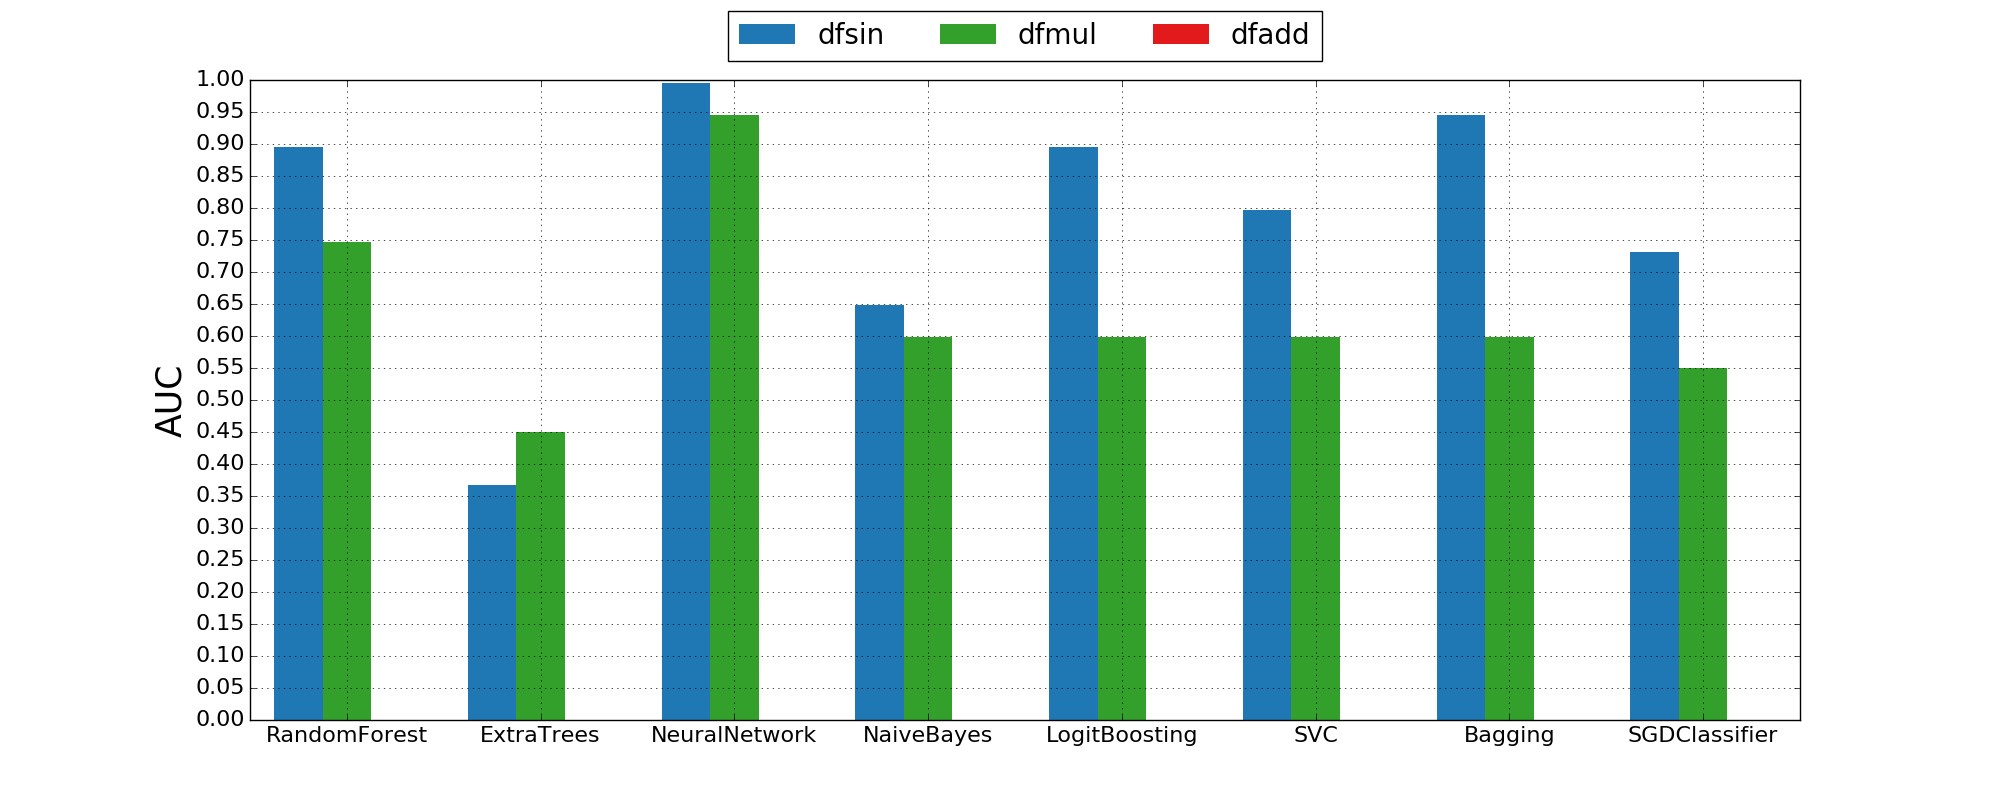
\includegraphics[scale=0.3]{DSPBlocks_auc_plot.png}
\caption{AUC bar chart for DSP Blocks}
\label{figure:dsp_auc_plot}
\end{figure}

Figure \ref{figure:dsp_auc_plot} showed the AUC score for all algorithms that are used to classify DSP blocks. The classification performance of all algorithms for DSP Blocks have the similar analogy as the ALUTs classification with NeuralNetwork being the top classifiers among the eight.

\section{Classification of Memory Bits}
\begin{figure}[h!]
\centering
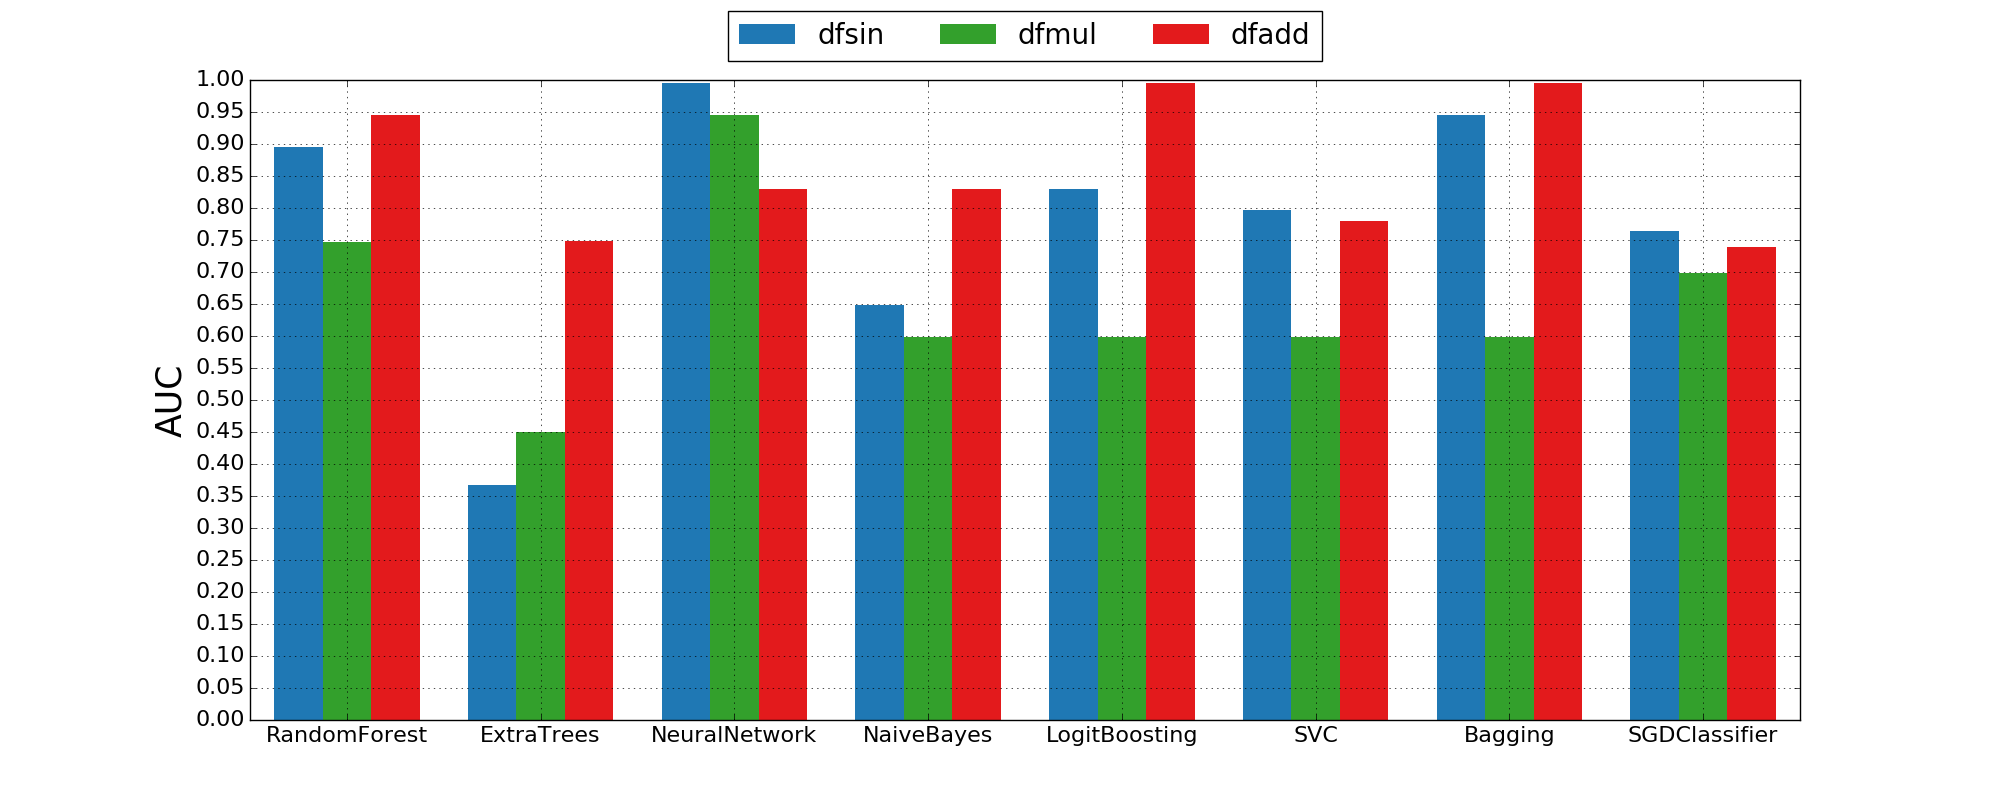
\includegraphics[scale=0.3]{MemoryBits_auc_plot.png}
\caption{AUC bar chart for Memory Bits}
\label{figure:MemoryBits_auc_plot}
\end{figure}

Figure \ref{figure:MemoryBits_auc_plot} showed the AUC score for all algorithms that are used to classify Memory Bits. Similar pattern to the classification of ALUTs can be found in this as well. NeuralNetwork classifier scored the average AUC score of 0.92. NaiveBayes, LogicBoosting, SVC, Bagging and SGDClassifier performed consistent as the same with the classification of ALUTs, Logic Utilization, DSP Bloacks and Memory Bits.

\section{Classification of Registers}
\begin{figure}[h!]
\centering
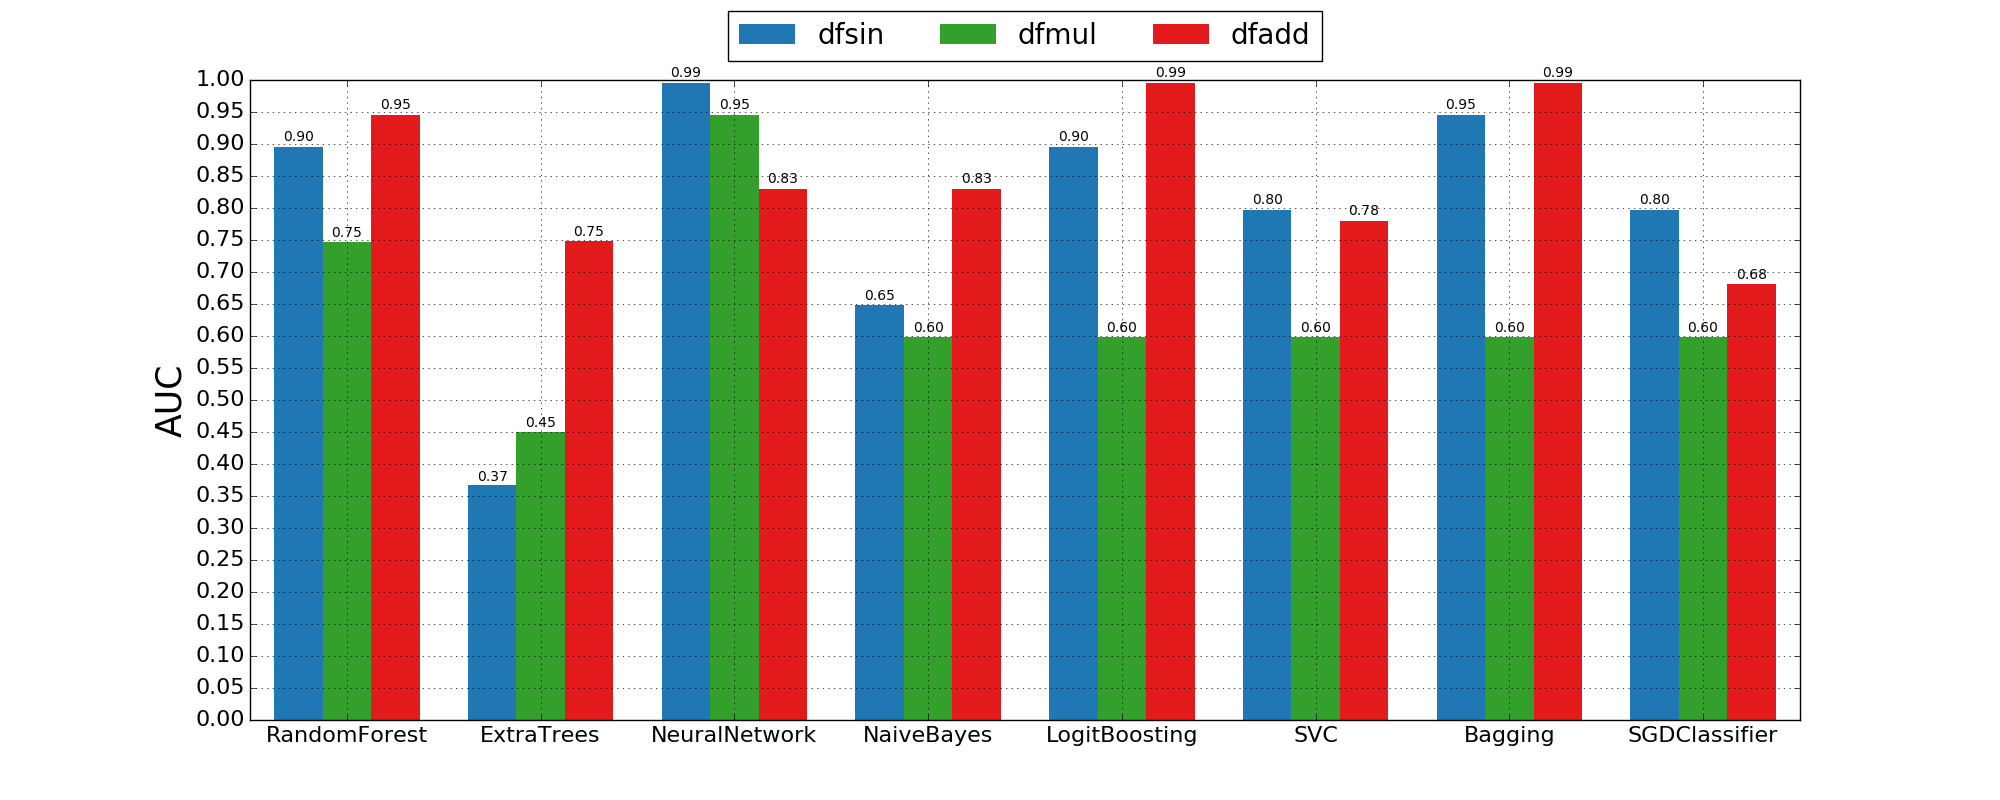
\includegraphics[scale=0.3]{Registers_auc_plot.png}
\caption{AUC bar chart for Registers}
\label{figure:Registers_auc_plot}
\end{figure}

Figure \ref{figure:Registers_auc_plot} showed the AUC score for all algorithms that are used to classify Registers. The same pattern arised in the classification of Registers compared with the aforementioned results. NeuralNetork scored the highest with the average AUC of 0.92.

\section{Classification of RAM Blocks}

\begin{figure}[h!]
\centering
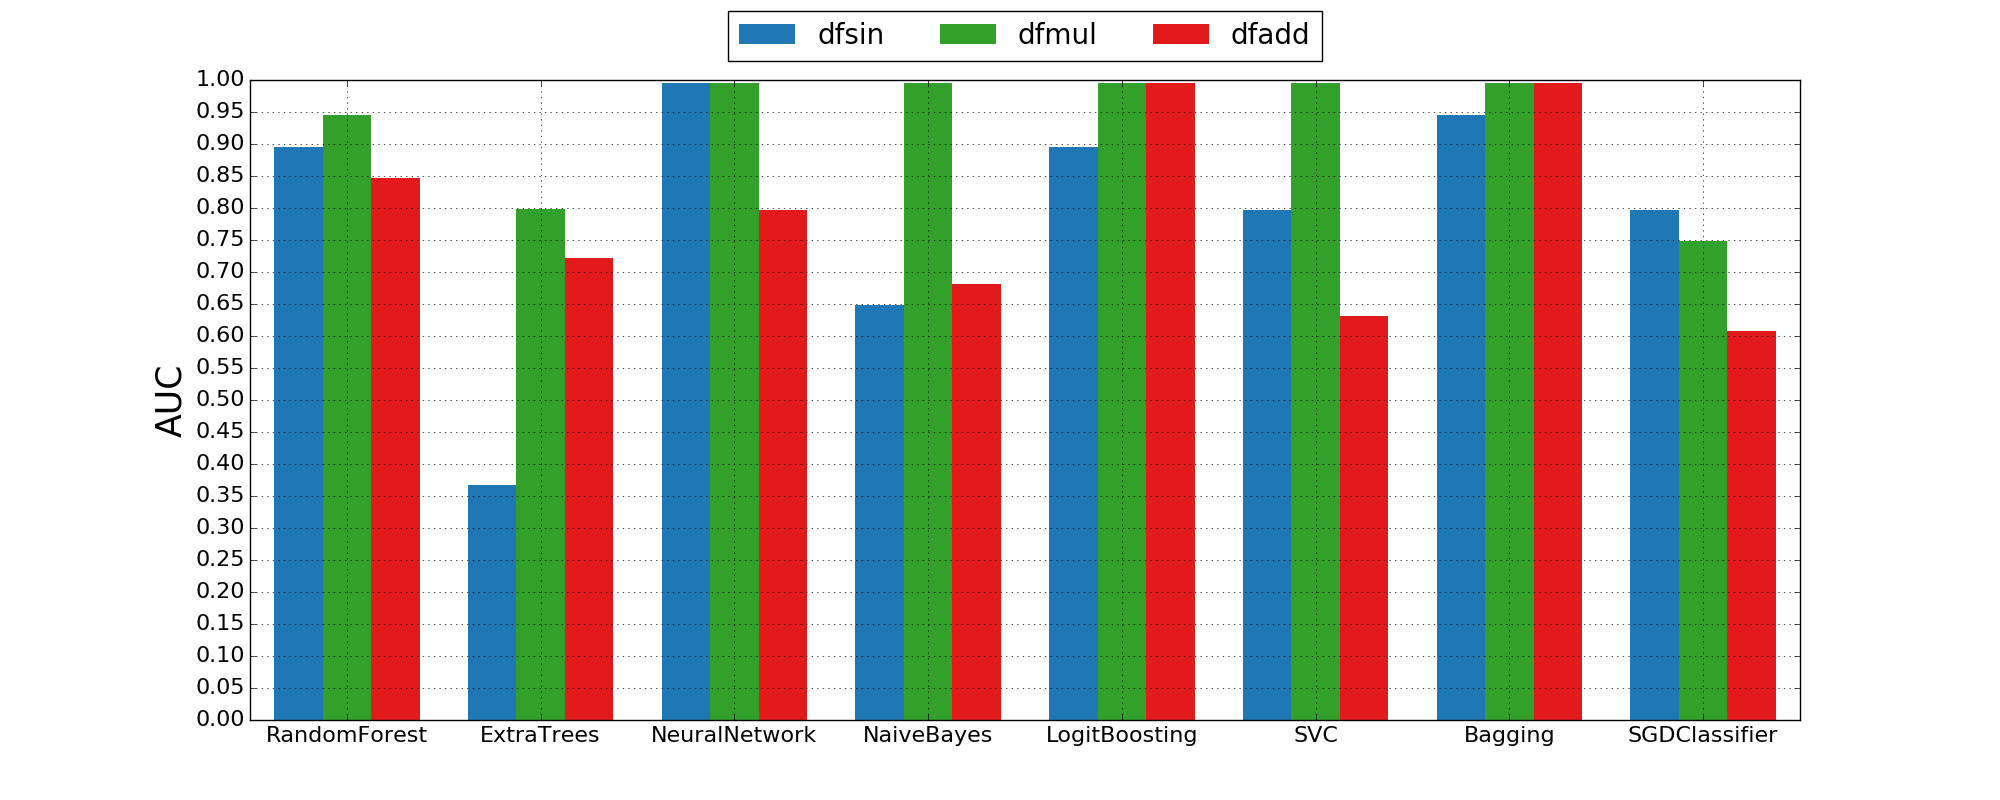
\includegraphics[scale=0.3]{RAMBlocks_auc_plot.png}
\caption{AUC bar chart for RAM Blocks}
\label{figure:RAMBlocks_auc_plot}
\end{figure}

Figure \ref{figure:RAMBlocks_auc_plot} showed the AUC score for all algorithms that are used to classify RAM Blocks. In this classification, NeuralNetwork was topped by Bagging and LogitBoosting classifiers. The average AUC score for Bagging and LogitBoosting classifiers are 0.98 and 0.95 respectively.

\section{Classification of Kernel Fmax}

\begin{figure}[h!]
\centering
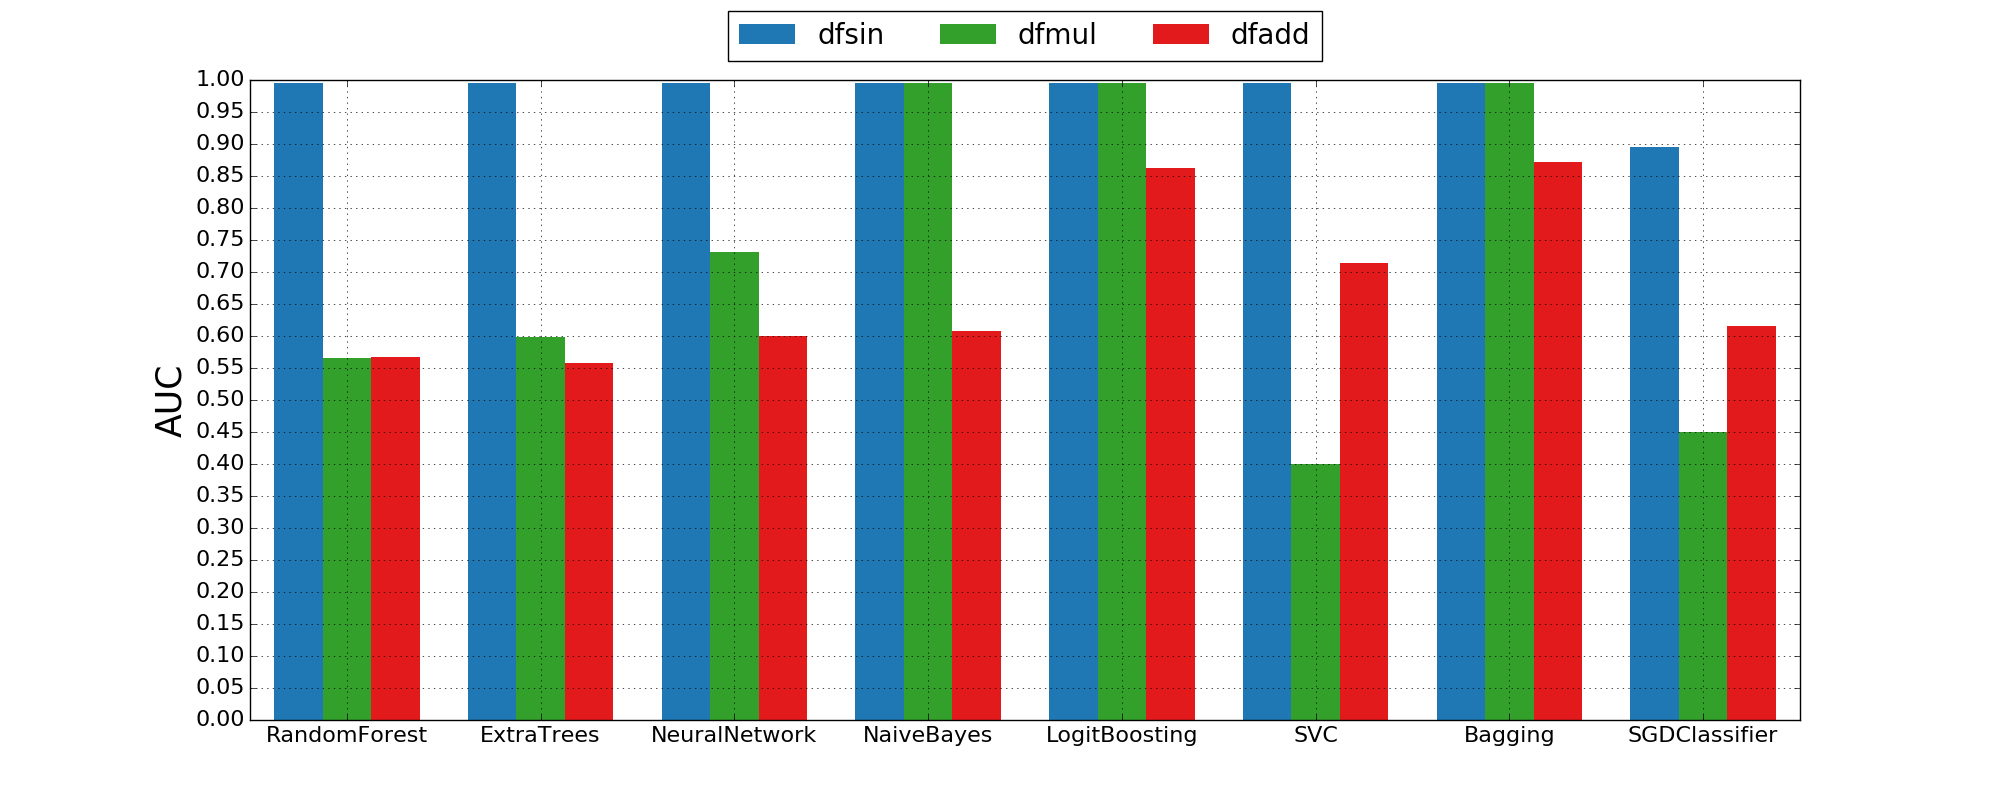
\includegraphics[scale=0.3]{KernelFmax_auc_plot.png}
\caption{AUC bar chart for Kernel Fmax}
\label{figure:kernelfmax_auc_plot}
\end{figure}

Figure \ref{figure:kernelfmax_auc_plot} showed the AUC score for all algorithms that are sued to classify Kernel Fmax. In this classification, RandomForest and ExtraTress classifier performed the same though we have seen that RandomForest performed better in the previous six classifications. Bagging and LogitBoosting performed the same in this classification with the average AUC score of 0.95.
